\documentclass[11pt]{article}
\usepackage[a4paper,margin=2.6cm]{geometry}
\usepackage[T1]{fontenc}
\usepackage[utf8]{inputenc}
\usepackage[english]{babel}
\usepackage{lmodern}
\usepackage{microtype}
\usepackage{amsmath,amssymb,amsthm}
\usepackage{booktabs,array}
\usepackage{enumitem}
\usepackage{listings}
\usepackage{xcolor}
\usepackage{tikz}
\usetikzlibrary{arrows.meta,positioning,fit,backgrounds,calc}
\usepackage[hidelinks]{hyperref}
\usepackage[export]{qam}
\usepackage{qam-physics}

\newtheorem{theorem}{Theorem}
\newtheorem{proposition}[theorem]{Proposition}
\newtheorem{corollary}[theorem]{Corollary}
\theoremstyle{definition}
\newtheorem{definition}{Definition}
\theoremstyle{remark}
\newtheorem*{remark}{Remark}

\lstset{basicstyle=\ttfamily\small,columns=fullflexible,keepspaces=true,breaklines=true,
  frame=single,framesep=4pt,rulecolor=\color{black!30},xleftmargin=6pt,xrightmargin=6pt}
\setlength{\emergencystretch}{3em}
\newcommand{\st}[1]{\textsf{#1}}
\newcommand{\cont}{\textsf{continue}}
\newcommand{\guard}{\textsf{guard}}
\newcommand{\reject}{\textsf{reject}}
\newcommand{\diag}{\operatorname{diag}}
\newcommand{\tr}{\operatorname{tr}}

\title{What a Conclusion Rests On:\\[2pt]
\large Checked Bookkeeping of Status, Inputs and Frames in Long Research Records}
\author{Marc Brendecke\\ \small Independent researcher, Bochum}
\InputIfFileExists{release-info}{}{\def\releaseline{Draft, \today}}
\date{\releaseline}

\begin{document}
\maketitle

\begin{abstract}
\noindent
When a research project is carried out over months with the help of language models, its written record grows faster than anyone
can check the dependencies inside it. The costly mistakes are then rarely wrong calculations. They are silent transitions: a result
that holds only under a condition is later cited as proved, a value that was put in by hand is later presented as derived, or two
quantities from different frames of reference are compared as if they were the same kind of thing. This article presents QAM, a small
typed bookkeeping language for such records, together with the tools that check it. Every statement in a QAM record carries a frame,
a status on a five-step scale from \st{open} to \st{proved}, the inputs it rests on and the exact versions of its premises. Four rules
guarantee, as the article proves, that no conclusion is stronger than what it rests on and that no input disappears along
a chain of reasoning; that frames change only through declared maps is enforced on every line and proved for a tree model of
derivations. Calculations are submitted as requests to an executor that
answers with one of three outcomes (\cont, \guard\ or \reject) and stores a hashed receipt; a premise graph in SQLite answers what
a result rests on and what depends on a given premise. A single worked example from elementary electrodynamics, a field
configuration observed before and after a Lorentz boost, runs through the whole article. QAM secures the form of a record. It does
not make its content true, and it replaces neither a proof assistant nor an experiment.
\end{abstract}

\section{Introduction}\label{sec:intro}

\subsection{Silent transitions}

A language model can produce more pages of mathematical text in an afternoon than a careful reader can check in a week. The errors
that matter in such a body of text are usually not the obvious ones. A sign error or a wrongly expanded bracket tends to surface at the
next calculation that uses it. Much harder to see are steps that leave no trace in the prose at all. We call them \emph{silent
transitions}, and three kinds recur:
\begin{itemize}[leftmargin=1.5em]
\item \emph{Promotion.} A statement that holds only under a stated condition, or that was only checked numerically, is cited a few
pages later as if it were a theorem, and further results are built on it.
\item \emph{An input read as a result.} A value that was taken from the literature, fitted to data or simply chosen reappears later
as a prediction of the theory.
\item \emph{Frame mixing.} Two quantities are compared or combined although they belong to different frames of description (different
observers, conventions, units, or model assumptions), and no map between those frames has been stated.
\end{itemize}
None of these is an arithmetic error, and each is a natural thing for a language model to do. A model continues a text so that it reads
coherently. A condition that was mentioned twenty paragraphs earlier contributes little to the coherence of the next sentence, so the
continuation smooths it away. This is not a rare malfunction but the expected behaviour of a system trained to continue text fluently.
Human authors do the same under time pressure; language models simply do it at scale.

We call the underlying problem \emph{premise drift}: over a long record, the premises on which a statement actually rests
drift away from the premises the text claims for it. Rewording does not reveal drift, because rewording is exactly how it happens.
What is needed is a structure outside the prose that records what each statement rests on and that cannot be changed by
rephrasing.

\subsection{What this article offers}

This article describes such a structure, called QAM, and the software that checks it. QAM grew out of a long, language-model-assisted
research project in mathematical physics~\cite{repo}, but nothing in it depends on that project, and this article assumes no
knowledge of it. Everything needed to understand the system, including the proofs of its properties, is contained here.

The contributions are:
\begin{enumerate}[leftmargin=1.5em]
\item A \emph{model} of research records (Section~\ref{sec:model}): an append-only sequence of typed entries, each with a frame, a
status, a set of inputs and a list of premises, and four rules that every entry must satisfy.
\item \emph{Proofs} of what the rules guarantee for whole records (Section~\ref{sec:properties}): no conclusion is ever stronger than
anything it rests on, however long the chain; inputs are never lost and never invented; frames change only through declared maps;
and a hash chain binds every conclusion to the exact versions of its premises. The core statements are also machine-checked in Lean~4
(Appendix~\ref{app:lean}).
\item \emph{Frames as an interface} (Section~\ref{sec:frames}): ordinary formulas are written in ordinary notation, but each one is
registered under a declared frame and interpretation, and moving it to another frame requires an explicit, declared step.
\item \emph{Tools} that check a record independently of one another: a \LaTeX{} package that refuses to typeset a record that breaks
the rules, a Lean program that checks the exported record against the same rules, and a script that recomputes all hashes (Section~\ref{sec:latex}).
\item An \emph{execution layer} (Sections~\ref{sec:requests}--\ref{sec:tape}): calculations are submitted as requests to an executor
that answers with one of three outcomes and stores a hashed receipt; a premise graph answers what a result rests on and what
depends on a premise; and a small tape machine is executed both in software and in two hardware descriptions as a cross-check.
\end{enumerate}

\subsection{Two design principles}

Two old ideas from computing shaped the design, and we state them because they explain decisions that would otherwise look
arbitrary.

The first is Konrad Zuse's separation of the arithmetic unit from the plan it executes~\cite{rojas97,bauer72}. Zuse's Z3 carried out
whatever the punched film prescribed; his Plankalk\"ul described computations independently of any machine, with separate classes of
variables for inputs and results. QAM adopts the same division of roles. The language model, like a computer algebra system or a
simulator, is the \emph{arithmetic unit}: it may formulate, transform and calculate. Which statements exist, what status they have and
what they rest on is the \emph{plan}, and the plan is a record that separate checkers read. Inputs and derived results are different
kinds of entry, just as Zuse's input and result variables were.

The second is Alan Turing's insight that not every question can be decided mechanically~\cite{turing36}. A checking system that knows
only ``valid'' and ``invalid'' must therefore either reject everything it cannot decide or quietly accept it. QAM gives the undecided
case its own outcome, the \emph{guard}: an open condition that is stored, hashed and inherited by everything built on it, rather than
smoothed away.

\subsection{How to read this article}

Section~\ref{sec:example} introduces a small worked example from electrodynamics that is used throughout. Sections~\ref{sec:model}
and~\ref{sec:properties} give the model and prove its properties. Sections~\ref{sec:frames} to~\ref{sec:llm} describe the tools, each
introduced on the same example. Section~\ref{sec:related} relates QAM to proof assistants, truth maintenance and provenance, and
collects the limitations. Commands for reproducing every result are collected in Appendix~\ref{app:repro}; the text itself avoids them
where it can.

\section{A worked example first}\label{sec:example}

Before defining anything, we look at a small calculation that has all the features QAM is meant to manage: two frames of description,
a map between them, an assumption about the set-up, a measurement, and an exact result. The physics is elementary and fully derived
here; the reader needs only the transformation law of electric and magnetic fields under a Lorentz boost. We use units with $c=1$.

\subsection{A field configuration and its Gram register}

In a laboratory frame, which we call \emph{Lab}, consider an electric field and a magnetic field of the form
\begin{equation}\label{eq:prep}
E = 2\,e_x,\qquad B = t\,e_y + u\,e_z,\qquad t^2+u^2 = 1 .
\end{equation}
The magnetic field has unit length and lies in the $yz$-plane; the number $t\in[-1,1]$ fixes its orientation. Put the two fields
side by side as the columns of a $3\times2$ matrix $F=[E\mid B]$. Its Gram matrix and the normalised Gram matrix are
\[
G = F^{\mathsf T}F = \begin{pmatrix} |E|^2 & E\cdot B\\ E\cdot B & |B|^2\end{pmatrix},\qquad
\rho = \frac{G}{\tr G}.
\]
We call $\rho$ the \emph{Gram register}: a positive matrix with unit trace that records the relative strengths of the two fields and
the angle between them, but forgets their overall scale and their orientation in space. For every field~\eqref{eq:prep} we have
$E\cdot B=0$, $|E|^2=4$ and $|B|^2=1$, so
\begin{equation}\label{eq:rho-lab}
\rho = \diag\bigl(\tfrac45,\tfrac15\bigr)\qquad\text{for every } t\in[-1,1].
\end{equation}

\subsection{The same fields seen by a moving observer}

A second observer moves with speed $v$ along the $z$-axis. We call that observer's frame \emph{Boosted}. With
$\gamma=(1-v^2)^{-1/2}$ the fields transform as
\[
\begin{aligned}
E'_x&=\gamma(E_x-vB_y), & E'_y&=\gamma(E_y+vB_x), & E'_z&=E_z,\\
B'_x&=\gamma(B_x+vE_y), & B'_y&=\gamma(B_y-vE_x), & B'_z&=B_z .
\end{aligned}
\]
For the fields~\eqref{eq:prep} this gives
\[
E' = \gamma\,(2-vt)\,e_x,\qquad B' = \gamma\,(t-2v)\,e_y + u\,e_z .
\]
We fix $v=\tfrac14$, so $\gamma^2=\tfrac{16}{15}$. The two boosted fields are still orthogonal. With
\[
A(t) = \bigl(2-\tfrac t4\bigr)^2
\]
we find $|E'|^2=\gamma^2A(t)$ and, using $u^2=1-t^2$,
\[
|B'|^2 = \gamma^2\bigl(t-\tfrac12\bigr)^2 + 1 - t^2 = \gamma^2\Bigl(A(t)-\tfrac{45}{16}\Bigr).
\]
The common factor $\gamma^2$ cancels in the normalisation, and the Gram register in the boosted frame is
\begin{equation}\label{eq:rho-boosted}
\rho' = \diag(p,\,1-p),\qquad p(t)=\frac{A(t)}{2A(t)-\frac{45}{16}}=\frac{(8-t)^2}{2(8-t)^2-45}.
\end{equation}
The denominator is at least $2\cdot 49-45=53$, so $p$ is well defined on $[-1,1]$.

\subsection{The point of the example}

Evaluate~\eqref{eq:rho-boosted} at the two ends of the range. For $t=1$ we get $p=49/53$, and for $t=-1$ we get $p=81/117=9/13$.
Both fields had the \emph{same} Gram register~\eqref{eq:rho-lab} in the Lab frame, but they have \emph{different} Gram registers in
the Boosted frame. Hence there is no function $f$ with $\rho'=f(\rho)$: a map from Lab registers to Boosted registers does not exist.
The boost acts on the fields; the register has forgotten the orientation that the boost needs.

This is precisely the kind of fact that is easy to lose in prose. A sentence such as ``the boost maps the Lab register to the Boosted
register'' sounds harmless and is false. In QAM, the map between the two frames is declared on the full description of the
fields, and every statement about the Boosted frame names the Lab statement and the map it came from. Section~\ref{sec:frames}
shows how; it also shows how adding the missing orientation and scale to the register restores a well-defined map.

\subsection{A measurement narrows the prediction}

Suppose we know nothing about $t$. Then all values of $p$ between the two endpoints can occur. To see that they all do, note that
$A$ decreases as $t$ grows (since $2-t/4>0$) and that
\[
\frac{dp}{dA} = -\frac{45/16}{\bigl(2A-45/16\bigr)^2} < 0,
\]
so $p$ is continuous and strictly increasing in $t$. Its range over $t\in[-1,1]$ is therefore the interval $[9/13,\,49/53]$, of width
about $0.232$.

Now suppose a measurement in the Lab frame tells us that $t=B\cdot e_y$ lies in $[-\tfrac14,\tfrac14]$. By monotonicity, the
prediction for the boosted frame is the image of the endpoints:
\begin{equation}\label{eq:interval}
p(-\tfrac14)=\frac{(33/4)^2}{2(33/4)^2-45}=\frac{121}{162},\qquad
p(\tfrac14)=\frac{(31/4)^2}{2(31/4)^2-45}=\frac{961}{1202},
\end{equation}
so $p\in[121/162,\,961/1202]$, an interval of width about $0.0526$, less than a quarter of the original one. This is a deterministic
constraint: no probability distribution over $t$ is assumed.

\subsection{What the example asks of a record}

The calculation is short, but a record of it has to keep several things apart:
\begin{itemize}[leftmargin=1.5em]
\item The preparation~\eqref{eq:prep} and the boost speed $v=\frac14$ are \emph{assumptions} about the set-up. Every conclusion
holds only under them.
\item The interval $t\in[-\frac14,\frac14]$ is a \emph{measured input}. The narrowed prediction~\eqref{eq:interval} rests on it and
must never be cited as if it followed from the theory alone.
\item Statements~\eqref{eq:rho-lab} and~\eqref{eq:rho-boosted} live in \emph{different frames}. They may be compared only through
the declared map that the boost provides, and that map acts on fields, not on registers.
\end{itemize}
These are exactly the three silent transitions of Section~\ref{sec:intro}. The rest of the article shows how QAM records them and
what it can and cannot guarantee about the record.

\section{The model}\label{sec:model}

This section defines QAM without reference to any tool. The \LaTeX{} package, the Lean checker and the database of later sections
are implementations of this model and apply the same rules.

\subsection{Records, frames and maps}

\begin{definition}[Record]
A \emph{record} is a finite sequence of entries $e_1,\dots,e_n$. It is extended only at the end (\emph{append-only}); an existing
entry is never changed. A correction is a new entry that names the entry it replaces.
\end{definition}

A \emph{frame} is the name of a frame of description: an observer, a convention, a choice of units, a model assumption, a sector of a
theory. Frames have no internal structure in the model. QAM knows only their names and the maps declared between them. A \emph{map}
$g\colon A\to B$ is a declared name with a source frame and a target frame; two maps can be declared to compose to a third. One
frame, written $*$, is reserved for convention-free statements such as a pure number or a theorem of mathematics; it is compatible
with every frame. If an application has several independent convention axes (say, an observer and a choice of units), each
combination gets a frame of its own, with maps between them.

In the example of Section~\ref{sec:example} there are two frames, Lab and Boosted, and one map, the boost along $z$, which we
call $\mathit{lorentz}_z\colon\mathrm{Lab}\to\mathrm{Boosted}$.

\subsection{Entries}

\begin{definition}[Entry]\label{def:entry}
A statement entry is a tuple
\[
e=(\mathit{kind},\ \mathit{key},\ \mathit{frame},\ \mathit{status},\ \mathit{inputs},\ \mathit{premises},\ \mathit{statement})
\]
where
\begin{itemize}[nosep,leftmargin=1.5em]
\item $\mathit{kind}$ is one of \texttt{input}, \texttt{claim}, \texttt{thesis}, \texttt{derive}, \texttt{convert};
\item $\mathit{key}$ is a name that is unique in the record;
\item $\mathit{frame}$ is a declared frame;
\item $\mathit{status}$ is taken from the totally ordered set
\[
\st{open}<\st{reading}<\st{conditional}<\st{computed}<\st{proved};
\]
\item $\mathit{inputs}$ is the set of input keys the entry rests on;
\item $\mathit{premises}$ is the list of earlier entries it was obtained from (for \texttt{convert}, together with the map used);
\item $\mathit{statement}$ is an optional text.
\end{itemize}
\end{definition}

The five kinds have fixed meanings. An \emph{input} is a value put in from outside: a measurement, a value from the literature, a
fitted parameter. A \emph{claim} is a statement without premises in the record, such as a cited theorem or an assumption. A
\emph{thesis} is a claim whose wording is part of its identity; a piece of work typically starts from one. A \emph{derivation} obtains
a statement from premises in the same frame, and a \emph{conversion} carries a statement into another frame through a declared map.
Two further entries carry no status: a \emph{comparison} of two entries, and a \emph{declaration of independence}, which asserts
that an entry rests on no input.

The status levels mean, from strongest to weakest: \st{proved}, established by proof; \st{computed}, supported by a calculation but
not proved; \st{conditional}, valid under named conditions that are not discharged; \st{reading}, an interpretation or assignment,
for instance the identification of a mathematical object with a physical quantity; \st{open}, not established. The author assigns
the status. The model does not check whether something declared \st{proved} has in fact been proved. It checks only whether a
conclusion is declared stronger than what it rests on.

In the example, the preparation~\eqref{eq:prep} together with the boost speed is a thesis (a claim with fixed wording) in Lab with status \st{conditional}: it is an
assumption about the experiment. The measured interval for $t$ is an input in Lab. The narrowed prediction~\eqref{eq:interval} is
obtained by first deriving, in Lab, a statement from the preparation and the measurement, and then converting it to Boosted through
$\mathit{lorentz}_z$.

\subsection{Rules}

\begin{definition}[Well-formed record]\label{def:rules}
A record is \emph{well formed} if every entry $e_i$ satisfies:
\begin{enumerate}[nosep,label=(R\arabic*),leftmargin=2.5em]
\item \emph{Declaration before use.} Every key, frame and map that $e_i$ mentions is declared in $e_1,\dots,e_{i-1}$, and no key is
declared twice.
\item \emph{No promotion.} If $e_i$ is a derivation or conversion with premises $p_1,\dots,p_m$, then
$\mathit{status}(e_i)\le\min_j\mathit{status}(p_j)$.
\item \emph{Inputs are preserved.} An input has $\mathit{inputs}=\{\mathit{key}\}$; a claim and a thesis have
$\mathit{inputs}=\emptyset$; for a derivation or conversion, $\mathit{inputs}(e_i)=\bigcup_j\mathit{inputs}(p_j)$. A declaration of
independence for $e$ is admissible only if $\mathit{inputs}(e)=\emptyset$.
\item \emph{No frame mixing.} The premises of a derivation and the two sides of a comparison lie in the same frame (or in $*$). A
conversion $\mathrm{convert}(g,p)$ with $g\colon A\to B$ requires $\mathit{frame}(p)=A$ and has frame $B$.
\end{enumerate}
\end{definition}

The three substantive rules answer the three silent transitions: (R2) prevents promotion, (R3) prevents an input from passing as a
result, and (R4) prevents frame mixing. (R1) makes it possible to check a record in a single pass from top to bottom.

In the example, (R2) forbids declaring the narrowed prediction \st{proved}, because it rests on a \st{conditional} preparation. (R3)
makes the measured input appear in the input set of the prediction, so that a declaration that the prediction is independent of
inputs is rejected. (R4) forbids comparing the Lab register~\eqref{eq:rho-lab} directly with the Boosted register~\eqref{eq:rho-boosted}.
Section~\ref{sec:latex} shows the actual error messages.

\subsection{Open conditions}\label{sec:open}

The stored fields determine, for every statement, what it ultimately rests on. We use the following terminology.

\begin{definition}[Open conditions]\label{def:open}
The \emph{open conditions} of an entry $e$ are the entries reachable from $e$ along premises whose status is below \st{proved},
together with $\mathit{inputs}(e)$.
\end{definition}

This is a reading of the stored structure, not an additional field. Section~\ref{sec:properties} proves that open conditions are
\emph{inherited}: a statement that rests on anything below \st{proved} is not \st{proved} itself, and every input remains visible however
many steps are taken.
An open condition therefore cannot disappear because further conclusions are built on top of it. Open conditions are objects of the
dependency graph, not remarks in the prose.

\subsection{Identity through a hash chain}

\begin{definition}[Entry hash]\label{def:hash}
The hash of an entry is
\[
h(e)=\mathrm{MD5}\bigl(\mathit{kind};\mathit{key};\mathit{frame};\mathit{status};\mathit{inputs};\mathit{sources};\mathit{statement}\bigr),
\]
where $\mathit{sources}$ is the list of the hashes of the premises of $e$. The hash of the record is the MD5 of the sequence of all
entry hashes.
\end{definition}

Because the hashes of the premises enter the hash of a conclusion, every conclusion names the exact versions of what it rests on. If
one word of a thesis changes, every hash that depends on it changes; independent entries keep theirs. Equal hashes mean equal
entries, not true ones. MD5 serves here to detect accidental change, not deliberate forgery; a release adds SHA-256 sums over the
source, the typeset document and the exported record.

\subsection{What the model leaves out}

The model has no semantics for statements. It does not know what a formula means, whether a calculation is right, or whether a frame
was chosen sensibly. Maps carry no status: if the justification of a map between two frames is itself a condition, it must be recorded
as an entry of its own. A claim declared \st{proved} without premises is accepted as such. A fitted value that is declared again under
a new name as a claim is not recognised as an input. These limits are deliberate. They keep the model small enough that its rules can
be checked completely and mechanically, by a compiler as well as by a proof assistant.

\section{What the rules guarantee}\label{sec:properties}

The rules of Definition~\ref{def:rules} are local: each one looks at a single entry and its immediate premises. What one wants to know
about a long record is global: whether a conclusion fifty steps down a chain still carries every condition and every input from the top.
This section shows that the local rules are enough. The proofs are short, and that is the point: the rules are precise enough to be
checked by a compiler and by a proof assistant alike. Appendix~\ref{app:lean} lists the corresponding machine-checked statements.

\subsection{Checking a record in one pass}

We model a checker that reads a record line by line. Its state $S$ is a finite map from keys to the stored information
$S(k)=(\mathit{frame},\mathit{status},\mathit{inputs},\mathit{prem})$, together with the declared maps. Reading a line either fails or
extends the state:
\begin{itemize}[leftmargin=1.5em]
\item an \emph{input} $k$ is accepted if $k$ is new, and stored with $\mathit{inputs}=\{k\}$ and no premises;
\item a \emph{claim} or \emph{thesis} $k$ is accepted if $k$ is new, and stored with no inputs and no premises;
\item a \emph{derivation} $k$ with premises $p_1,\dots,p_m$ ($m\ge1$) is accepted if $k$ is new, every $p_j$ is stored, lies in the
frame of $k$ or in $*$, has status at least that of $k$, and the declared inputs of $k$ are exactly the union of the inputs of the $p_j$;
\item a \emph{conversion} $k=\mathrm{convert}(g,p)$ is accepted if $k$ is new, $g\colon A\to B$ is declared, $p$ is stored in frame $A$,
$k$ is in frame $B$, $k$ is not stronger than $p$, and the inputs of $k$ are those of $p$;
\item a \emph{comparison} or \emph{declaration of independence} is accepted if (R4), respectively (R3), holds for it; it does not change the state;
\item a \emph{map declaration} is accepted if the name of the map is new.
\end{itemize}
A record is \emph{accepted} if every line is accepted in turn, starting from the empty state. This is exactly the procedure of the
Lean checker of Section~\ref{sec:latex}, and it is the reason for rule (R1): because nothing may be used before it is declared, a single
pass suffices.

\subsection{An invariant of accepted records}

\begin{definition}[Good state]\label{def:good}
A state $S$ is \emph{good} if for every stored key $k$ with $S(k)=(f,s,I,P)$:
\begin{enumerate}[label=(\alph*),nosep,leftmargin=2em]
\item every premise $p\in P$ is stored, with $S(p)=(f',s',I',P')$ such that $s\le s'$ and $I'\subseteq I$;
\item every $x\in I$ either is $k$ itself and $P$ is empty (that is, $k$ is an input), or lies in the inputs of some premise $p\in P$.
\end{enumerate}
\end{definition}

\begin{theorem}[Accepted records are good]\label{thm:good}
The state reached after an accepted record is good.
\end{theorem}

\begin{proof}
By induction on the number of lines. The empty state is good because it stores nothing. Suppose $S$ is good and a line is accepted,
giving $S'$. Comparisons, declarations of independence and map declarations leave the stored keys unchanged, so $S'$ is good. Otherwise
exactly one new key $k$ is added, and since $k$ was new, no earlier entry changes; the earlier entries still satisfy (a) and (b) in $S'$
because their premises are still stored with the same information. For the new key, (a) and (b) are exactly what the acceptance test
checked: an input has $I=\{k\}$ and no premises; a claim has neither; a derivation or conversion has stored premises of at least its
status whose inputs are contained in $I$, and every element of $I$ comes from some premise.
\end{proof}

\subsection{No promotion, at any distance}

Say that $a$ is an \emph{ancestor} of $k$ if $a$ can be reached from $k$ by following premises one or more times.

\begin{theorem}[No promotion]\label{thm:nopromotion}
In an accepted record, if $a$ is an ancestor of $k$ then $\mathit{status}(k)\le\mathit{status}(a)$.
\end{theorem}

\begin{proof}
Induction on the length of the path from $k$ to $a$. For a direct premise this is part (a) of Theorem~\ref{thm:good}. For a longer path
$k\to m\to\dots\to a$, the induction hypothesis gives $\mathit{status}(m)\le\mathit{status}(a)$, part (a) gives
$\mathit{status}(k)\le\mathit{status}(m)$, and the order on statuses is transitive.
\end{proof}

\begin{corollary}[Proved rests only on proved]\label{cor:proved}
In an accepted record, every ancestor of an entry with status \st{proved} has status \st{proved}. Equivalently, an entry with an ancestor
below \st{proved} is not \st{proved}.
\end{corollary}

\begin{proof}
\st{proved} is the top of the order, so $\st{proved}\le\mathit{status}(a)$ forces $\mathit{status}(a)=\st{proved}$.
\end{proof}

For the example: the narrowed prediction~\eqref{eq:interval} has the conditional preparation as an ancestor, two steps up. By
Theorem~\ref{thm:nopromotion} it can be at most \st{conditional}, however many further conclusions are later drawn from it.

\subsection{Inputs are never lost and never invented}

\begin{theorem}[Inputs]\label{thm:inputs}
In an accepted record:
\begin{enumerate}[label=(\roman*),nosep,leftmargin=2em]
\item if $a$ is an ancestor of $k$, then $\mathit{inputs}(a)\subseteq\mathit{inputs}(k)$;
\item every input of $k$ is $k$ itself (if $k$ is an input) or an input of one of its premises;
\item if $\mathit{inputs}(k)=\emptyset$, then no ancestor of $k$ has an input, and in particular no ancestor is an input entry.
\end{enumerate}
\end{theorem}

\begin{proof}
(i) Induction on the path, using part (a) of Theorem~\ref{thm:good} and transitivity of $\subseteq$. (ii) is part (b) of
Theorem~\ref{thm:good}. (iii) follows from (i): an ancestor with a non-empty input set would force $\mathit{inputs}(k)\neq\emptyset$;
and an input entry $a$ has $\mathit{inputs}(a)=\{a\}\neq\emptyset$.
\end{proof}

Part (iii) is what makes the declaration of independence meaningful. If a record declares that a result is independent of all inputs and
the record is accepted, then no measured or fitted value occurs anywhere above that result. In the example, the measurement is an
ancestor of the narrowed prediction, so the prediction carries it in its input set, and a declaration that the prediction is
independent of inputs is rejected.

\subsection{Frames change only through declared maps}

To state the frame property we look at a single conclusion and the tree of steps that produced it. A \emph{derivation tree} has
leaves (entries without premises) and three kinds of inner node: a step from one premise, a join of two premises, and a conversion
through a map $g$ into a frame $b$. A tree is \emph{well formed} relative to a set $D$ of declared maps if no node is stronger than
its children, the two children of a join lie in the same frame, and every conversion uses a map in $D$ whose source is the frame of its
child.

\begin{theorem}[Frames]\label{thm:frames}
In a well-formed tree, the frame of every leaf reaches the frame of the root through a chain of declared maps. If no maps are
declared, every leaf lies in the frame of the root.
\end{theorem}
\noindent The tree model has no convention-free frame; leaves in $*$, which the record checker admits as premises of any frame, are
excluded here. The frame property is proved for trees; the record checker enforces the corresponding local condition on every line.


\begin{proof}
Induction on the tree. A leaf reaches its own frame through the empty chain. A step keeps the frame of its child. For a join, both
children have the same frame, which is the frame of the join, and the induction hypothesis applies to each side. For a conversion
through $g\colon a\to b$, every leaf of the child reaches $a$ by induction, and appending $g$ gives a chain to $b$. If $D$ is empty, the
only chains are empty, so every leaf lies in the frame of the root.
\end{proof}

Theorem~\ref{thm:frames} is the formal content of rule (R4): there is no way to arrive in the Boosted frame from a Lab statement except
through $\mathit{lorentz}_z$ or another declared map.

\subsection{The hash chain binds conclusions to premises}

The checker also reads the hash and the list of source hashes recorded for every entry. It accepts the hash part of a line if the
entry's hash has not occurred before and, for a derivation or conversion, if the recorded sources are exactly the hashes recorded
earlier for its premises, in order; leaves must have no sources.

\begin{proposition}[Hash links]\label{prop:links}
In a record accepted by the hash check, the sources of every derivation and conversion are the hashes of its premises as they were
recorded, and no hash occurs twice. If, in addition, the hashes are computed as in Definition~\ref{def:hash} and no MD5 collision
occurs among the entries involved, then changing any field of an entry changes its hash and the hash of every entry of which it is an
ancestor, and leaves the hash of every other entry unchanged.
\end{proposition}

\begin{proof}
The first sentence is what the check tests, line by line. For the second, an entry's hash is computed from its own fields and the
hashes of its premises. Changing a field changes the hashed string and therefore, absent a collision, the hash. By induction along the
paths from the changed entry, every descendant receives a different source list and hence a different hash. An entry that is not a
descendant has the same fields and, by induction on the record, the same premise hashes, and hence the same hash.
\end{proof}

The proposition separates what is proved from what is assumed. That the links are consistent is checked. That a changed statement
yields a changed hash is a property of the hash function, which is assumed and not proved; MD5 is chosen to detect accidental change
and gives no protection against deliberate collisions.

\subsection{What the proofs do not say}

All results above are relative to what is declared. A record that declares a premise-free claim as \st{proved} is accepted, and so are
its consequences. A checked record shows that the stated statuses, inputs and frames are mutually consistent. It does not show that
any statement is true.

\section{Frames as an interface}\label{sec:frames}

The model of Section~\ref{sec:model} treats statements as opaque. In practice, most statements in a scientific record are formulas,
and a formula means something only within a frame: the same symbols denote different things for different observers, in different
units, or under different model assumptions. QAM therefore treats a frame as an \emph{interface} with two sides. On the right stands
the formula in ordinary notation, exactly as a physicist or mathematician would write it. On the left stand its roles: the frame, the
language or theory in which it is to be read, and its status. Inside a declared context the left side is implicit and the text looks like
any other paper. Outside that context, or when a formula is carried to another frame, the left side becomes visible.

\subsection{Profiles and contexts}

A \emph{profile} fixes one interpretation within one frame. It consists of a key, a frame, a language, a status and a short description
of the interpretation; once declared it cannot be changed. A \emph{context} selects a profile as the default for a stretch of text.
Formulas registered inside the context are stored with the profile as a premise. Because the profile is hashed together with its
description (Definition~\ref{def:hash}), changing the interpretation changes the hash of every formula registered under it.

The following lines appear in the source of this article. They register the two frames of the example, a profile for each, and the
first formula; the package checks them while the article is typeset.

\begin{lstlisting}
\qamframe{Lab}\qamframe{Boosted}
\qamprofile{lab}{Lab}{L_{\rm EM}}{conditional}{Laboratory fields and their Gram readouts}
\qamprofile{boosted}{Boosted}{L_{\rm EM}}{conditional}{Fields of an observer boosted along z, c=1}
\begin{qamcontext}{lab}
\[ \qamformula{field-pair}{conditional}{F_b=[2e_x\mid b\,e_y],\quad b\in\{+1,-1\}} \]
\end{qamcontext}
\end{lstlisting}

\qamframe{Lab}\qamframe{Boosted}
\qamprofile{lab}{Lab}{L_{\rm EM}}{conditional}{Laboratory fields and their Gram readouts}
\qamprofile{boosted}{Boosted}{L_{\rm EM}}{conditional}{Fields of an observer boosted along z, c=1}
\noindent Inside the context the formula prints as an ordinary display:
\begin{qamcontext}{lab}
\[
\qamformula{field-pair}{conditional}{F_b=[2e_x\mid b\,e_y],\quad b\in\{+1,-1\}}
\]
\[
\qamformula[field-pair]{gram-input}{conditional}{\rho(F_b)=\operatorname{diag}(4/5,1/5)}
\]
\end{qamcontext}
These are the two fields of the example with $t=b$ and $u=0$. Both have the same Gram register, as the second display records.
Outside the context, a reference to the stored formula shows its roles automatically; \verb|\qamphys{gram-input}| prints
\[
\qamphys{gram-input}
\]
so that a reader who meets the formula elsewhere sees in which frame and language it was stated.

\subsection{Explicit conversion}

A formula is carried to another frame only by an explicit step that names the declared map, the source formula, the target profile and
the target formula. The target formula is supplied by the author; QAM does not compute it.

\qammap[\Lambda_z]{lorentz-z}{Lab}{Boosted}
\begin{lstlisting}
\qammap[\Lambda_z]{lorentz-z}{Lab}{Boosted}
\[ \qamphysconvert{boosted-fields}{conditional}{lorentz-z}{field-pair}{boosted}
     {F'_b=\gamma\,[(2-vb)\,e_x\mid(b-2v)\,e_y]} \]
\end{lstlisting}
prints, with both sides of the interface visible,
\[
\qamphysconvert{boosted-fields}{conditional}{lorentz-z}{field-pair}{boosted}
  {F'_b=\gamma\,[(2-vb)\,e_x\mid(b-2v)\,e_y]}
\]
and the Gram registers in the new frame are then registered inside the Boosted context:
\begin{qamcontext}{boosted}
\[
\qamformula[boosted-fields]{gram-output}{conditional}
  {\rho(F'_{+1})\big|_{v=1/4}=\operatorname{diag}(49,4)/53,\qquad \rho(F'_{-1})\big|_{v=1/4}=\operatorname{diag}(9,4)/13}
\]
\end{qamcontext}
The record now states, in a form the checkers can follow, what Section~\ref{sec:example} found by hand: the conversion runs from
\texttt{field-pair}, the fields, and not from \texttt{gram-input}, the register. A conversion from the register would require a map
that does not exist, and nothing in the record claims one.

\subsection{Repairing the map by enriching the description}

The register lost exactly two pieces of information: the overall scale $n=\tr G$ and the orientation of the fields in space. Write
$D=(\rho,n,O)$ with $O\in SO(3)$, and reconstruct the fields as $F=O\,F_0(n\rho)$, where $F_0(G)$ is the upper-triangular
$3\times2$ matrix with $F_0^{\mathsf T}F_0=G$ (a Cholesky factor padded with a zero row). For the two fields above,
$G=\diag(4,1)$, $F_0=[2e_x\mid e_y]$, $n=5$ and $O=\diag(1,b,b)$, so $D_b=(\diag(\frac45,\frac15),5,\diag(1,b,b))$ and indeed
$OF_0=F_b$. The two inputs now differ in their orientation component. The composite ``reconstruct, boost, encode'' is a well-defined
map on such descriptions wherever the boosted field again has rank two, which holds for both fields at $v=\frac14$. In QAM it is
declared as a second map from Lab to Boosted, and the corresponding entries are conversions through it. The normalised output is
unchanged, because a common scale cancels in $\rho$; what has changed is that the record now contains a map that exists.

\subsection{What is checked and what is not}

The package checks that a context is open when a formula is registered, that profiles and formulas are not declared twice, that a
conversion uses a declared map whose source and target match the profiles involved, that two profiles in the same frame are not mixed
without an explicit step, and that status never rises (no target is stronger than its source or its target profile). It does not check
the formulas. They are stored as \TeX{} text, not as expressions of a computer algebra system, so the boost law, units, domains and the
truth of a conversion are not verified. Section~\ref{sec:requests} shows how calculations whose results matter are instead submitted to
an executor and stored with a receipt.

\section{The record in \LaTeX, and three independent checkers}\label{sec:latex}

Mathematical texts are written in \LaTeX, and language models write \LaTeX{} readily. The natural place to keep a record is therefore the
document itself: each statement is declared where it appears in the text, and the \TeX{} compiler applies the rules while it typesets.
The package \texttt{qam.sty} does this. It uses only the \LaTeX{} kernel (expl3, \LaTeX{} 2022-06 or later) and depends on no
application.

\subsection{Declaring the example}

The following block is part of the source of this article. It records the interval prediction of Section~\ref{sec:example}. The frames
and the map were declared in Section~\ref{sec:frames}; the optional first argument of each command is the symbol under which the entry
is displayed.

\begin{lstlisting}
\qamthesis[\mathcal P]{preparation}{Lab}{conditional}
  {E=2e_x, B=t e_y+u e_z, t^2+u^2=1, c=1, boost v=1/4 along z}
\qaminput[t_I]{measurement}{Lab}{conditional}
\qamconvert[p]{range-rule}{conditional}{lorentz-z}{preparation}
\qamderive[\mathcal P_I]{measured-preparation}{conditional}{preparation,measurement}
\qamconvert[p_I]{narrowed-range}{conditional}{lorentz-z}{measured-preparation}
\end{lstlisting}
\qamthesis[\mathcal P]{preparation}{Lab}{conditional}
  {E=2e_x, B=t e_y+u e_z, t^2+u^2=1, c=1, boost v=1/4 along z}
\qaminput[t_I]{measurement}{Lab}{conditional}
\qamconvert[p]{range-rule}{conditional}{lorentz-z}{preparation}
\qamderive[\mathcal P_I]{measured-preparation}{conditional}{preparation,measurement}
\qamconvert[p_I]{narrowed-range}{conditional}{lorentz-z}{measured-preparation}


\begin{figure}[t]
\centering
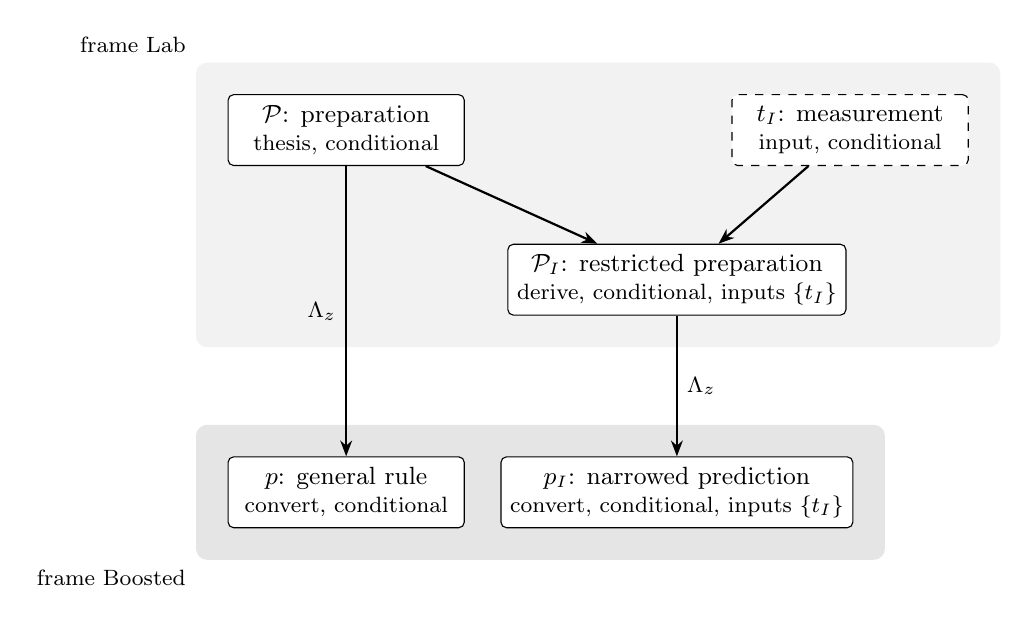
\begin{tikzpicture}[node distance=10mm and 14mm,
  box/.style={draw,rounded corners=2pt,align=center,font=\small,minimum width=30mm,minimum height=9mm,fill=white},
  inp/.style={box,dashed},
  arr/.style={-{Stealth[length=2mm]},thick}]
\node[box] (P) at (0,0) {$\mathcal P$: preparation\\[-1pt]\footnotesize thesis, conditional};
\node[inp] (T) at (6.4,0) {$t_I$: measurement\\[-1pt]\footnotesize input, conditional};
\node[box] (PI) at (4.2,-1.9) {$\mathcal P_I$: restricted preparation\\[-1pt]\footnotesize derive, conditional, inputs $\{t_I\}$};
\node[box] (p) at (0,-4.6) {$p$: general rule\\[-1pt]\footnotesize convert, conditional};
\node[box] (pI) at (4.2,-4.6) {$p_I$: narrowed prediction\\[-1pt]\footnotesize convert, conditional, inputs $\{t_I\}$};
\draw[arr] (P) -- (PI); \draw[arr] (T) -- (PI);
\draw[arr] (P) -- node[left,font=\footnotesize]{$\Lambda_z$} (p);
\draw[arr] (PI) -- node[right,font=\footnotesize]{$\Lambda_z$} (pI);
\begin{scope}[on background layer]
\node[fill=black!5,rounded corners,fit=(P)(T)(PI),inner sep=4mm,label={[font=\footnotesize]north west:frame Lab}] {};
\node[fill=black!10,rounded corners,fit=(p)(pI),inner sep=4mm,label={[font=\footnotesize]south west:frame Boosted}] {};
\end{scope}
\end{tikzpicture}
\caption{The record of the interval prediction. Arrows point from a premise to what is obtained from it; the two arrows labelled
$\Lambda_z$ are conversions through the declared boost map, the only way from the Lab frame to the Boosted frame. The dashed box is an
input. Its key travels down to every entry below it, so $p_I$ carries it, while $p$ does not.}
\label{fig:record}
\end{figure}

\noindent Figure~\ref{fig:record} shows the resulting graph. The thesis $\mathcal P$ is the preparation~\eqref{eq:prep} with $v=\frac14$; as a thesis, its wording is part of its
hash, so a change of the set-up changes every hash below it; the input $t_I$ is the measured interval
$t\in[-\frac14,\frac14]$; $p$ is the general rule~\eqref{eq:rho-boosted} in the Boosted frame; $\mathcal P_I$ is the preparation
restricted by the measurement; and $p_I$ is the narrowed prediction~\eqref{eq:interval}. The author states the status of each entry.
The frame and the inputs of a derivation are not stated but computed from the premises, so they cannot be stated wrongly.

From these declarations the package typesets a compact notation. \verb|\qam{narrowed-range}| and \verb|\qam{range-rule}| give
\begin{center}
\qam{narrowed-range}\qquad\qquad \qam{range-rule}
\end{center}
Here $\Lambda_z$ is the symbol declared for the boost map, the left superscript is the frame, ``$\Leftarrow$'' reads ``derived
from'', $R(w)$ is the readout of a witness $w$ (a value put in by hand), and $W$ lists the witnesses an entry rests on. Similarly,
\verb|\qamshow{narrowed-range}| gives the short form \qamshow{narrowed-range}. One reads off that $p_I$ was carried from Lab to Boosted,
rests on the measured input $t_I$ and holds at most conditionally, while the general rule $p$ rests on no input.

The package also prints a ledger of all entries. For the five entries above it reads:
\begin{center}
\small
\begin{tabular}{@{}lll@{}}
\toprule
key & QAM notation & hash\\
\midrule
\texttt{preparation} & \qam*{preparation} & \texttt{\qamhash{preparation}}\\
\texttt{measurement} & \qam*{measurement} & \texttt{\qamhash{measurement}}\\
\texttt{range-rule} & \qam*{range-rule} & \texttt{\qamhash{range-rule}}\\
\texttt{measured-preparation} & \qam*{measured-preparation} & \texttt{\qamhash{measured-preparation}}\\
\texttt{narrowed-range} & \qam*{narrowed-range} & \texttt{\qamhash{narrowed-range}}\\
\bottomrule
\end{tabular}
\end{center}
The full record of the article, including the entries of Section~\ref{sec:frames}, is reproduced in Appendix~\ref{app:record}.

\subsection{What happens when a rule is broken}

By default a violation stops the compiler. This is deliberate: a document containing a promotion should not come out as a PDF. Had the
last line above declared the prediction \st{proved}, typesetting would have stopped with
\begin{lstlisting}
! Package qam Error: Promotion: `narrowed-range' is declared `proved', but its
(qam)                weakest premise `measured-preparation' is only
(qam)                `conditional'.
\end{lstlisting}
A declaration that the prediction is independent of inputs, \verb|\qamindependent{narrowed-range}|, stops with
\begin{lstlisting}
! Package qam Error: `narrowed-range' is cited as independent of inputs, but
(qam)                it rests on: measurement.
\end{lstlisting}
and a direct comparison of the prediction with the preparation,
\begin{center}\verb|\qamcompare{narrowed-range}{preparation}|,\end{center}
stops with
\begin{lstlisting}
! Package qam Error: Frame mixing: `narrowed-range' (frame Boosted) and
(qam)                `preparation' (frame Lab) are compared without a
(qam)                declared map.
\end{lstlisting}
These messages were produced by compiling the three variants; they are quoted, not paraphrased. Further messages cover keys, frames and
maps that are used before they are declared or declared twice, unknown status names, a conversion whose map starts in the wrong frame,
and a derivation without premises. A warning mode (\texttt{mode=warning}) turns errors into warnings so that the package can be
introduced into an existing text; the record exported in that mode is then rejected by the Lean checker, so the violation cannot pass
unnoticed.

\subsection{The exported record}

With the option \texttt{export}, the package writes every entry as one line of a plain text file. For the example, the lines of the
prediction and its ancestors read (hashes shortened, lines wrapped)
\begin{lstlisting}
map lorentz-z : Lab -> Boosted
preparation := thesis; frame Lab; status conditional; inputs {};
    hash 839F0699...; sources {}; statement E=2e_x, B=t e_y+u e_z, ...
measurement := <6,measurement>; frame Lab; status conditional;
    inputs {measurement}; hash C2DEF159...; sources {}
measured-preparation := derive(preparation,measurement); frame Lab;
    status conditional; inputs {measurement}; hash 16E7B1C0...;
    sources {839F0699...,C2DEF159...}
narrowed-range := convert(lorentz-z,measured-preparation); frame Boosted;
    status conditional; inputs {measurement}; hash 3F78DEBD...;
    sources {16E7B1C0...}
\end{lstlisting}
An input is written as \texttt{<6,measurement>}: the format tags every value put in by hand as a \emph{witness}, one of a small
set of tagged object kinds that the request language of Section~\ref{sec:requests} also uses. Appendix~\ref{app:record} reproduces the full exported record of this article. The exported file is the interface to every other
checker. Checking does not depend on trusting the \TeX{} package.

\subsection{Three checkers}

Three programs, written independently of one another, check an exported record. Two of them apply the rules of
Definition~\ref{def:rules}; the third checks the hashes:
\begin{enumerate}[leftmargin=1.5em]
\item the \TeX{} package, while the document is typeset;
\item \texttt{qamcheck}, a program written in Lean~4, on the exported file. It performs the one-pass check of
Section~\ref{sec:properties}, including the hash links, and its correctness properties are proved in Lean (Appendix~\ref{app:lean});
\item \texttt{qamhash.py}, a short Python script that recomputes every entry hash, the record hash and the MD5 of the source file.
\end{enumerate}
Lean does not compute MD5; the script does. Lean checks that the links between the recorded hashes are consistent. For a release, a
manifest of SHA-256 sums over the source, the PDF and the record is written in addition.

A checker that only ever sees good records is not tested. The repository therefore contains deliberately broken records that must be
rejected: a promotion, a frame mixing, a false declaration of independence, a conversion whose map starts in the wrong frame, a broken hash
link, an entry whose statement was edited after export, and an input that was deleted by hand. The last cannot be produced by the \TeX{}
package at all. It ensures that the Lean checker does more than repeat what the package already prevents. The \TeX{} package has its
own test suite of 34 small documents, each of which must either compile or stop with a specific error.

\section{Calculations as requests}\label{sec:requests}

A record says what each statement rests on. It does not perform calculations. In a project carried out with language models, the
calculations are the part most likely to be invented: a model asked for a number will produce one. QAM therefore separates the request
for a calculation from its execution and from the stored result. Requests are written in a small request language, MML; they are
executed by an executor, MMA; and every execution leaves a \emph{receipt}.

\subsection{Three outcomes}

The central design decision is that an execution has three possible outcomes, not two:
\begin{itemize}[leftmargin=1.5em]
\item \cont: the request was admissible and was carried out; the receipt contains the result.
\item \guard: the request was well formed, but a condition it depends on is not available or not fulfilled, for example a premise that is not in the
record. No result is returned or stored. The receipt names the missing condition as an obligation.
\item \reject: the request itself is not admissible, for example because an argument lies outside the declared range.
\end{itemize}
A \guard\ is not a failure. It is the third outcome required by the decidability boundary of Section~\ref{sec:intro}: the honest answer
when a precondition is open. It is stored, hashed and retrievable like any other result.

\subsection{The example as a request}

The interval calculation of Section~\ref{sec:example} is available as an allowlisted recipe. A request names the recipe, the frames, the
preparation, the boost and the measured interval:
\begin{lstlisting}
{ "id": "gram_boost_interval", "instruction": "READOUT", "guards": [],
  "arguments": { "recipe": "em.gram-boost-range",
                 "preparation": "E2x-B-unit-yz", "frame": "Lab",
                 "target_frame": "Boosted", "boost": "z:1/4",
                 "a": "-1/4", "b": "1/4" } }
\end{lstlisting}
Before computing, the executor looks up the analytic rule the recipe depends on, by the hash of its record entry, and follows the
premises of that entry recursively. We ran the request four times, the first as shown and then with one thing changed each time:
\begin{center}
\small
\begin{tabular}{@{}p{0.34\textwidth}p{0.12\textwidth}p{0.45\textwidth}@{}}
\toprule
Request & Outcome & Receipt states\\
\midrule
as above, rule indexed & \cont & target interval $[121/162,\ 961/1202]$\\
rule not in the database & \guard & obligation: missing premise (the rule's hash)\\
interval with $a>b$ & \reject & error: endpoints must satisfy $-1\le a\le b\le 1$\\
boost $z{:}1/3$ instead of $z{:}1/4$ & \reject & error: the recipe requires the declared preparation and boost\\
\bottomrule
\end{tabular}
\end{center}
The first row reproduces the hand calculation~\eqref{eq:interval} with exact rational arithmetic. The second shows the guard: the same
request against a database in which the rule is not recorded returns no result, because the result would rest on something the record does
not contain. The third and fourth show that the recipe accepts only the situation for which the rule was derived; it does not
extrapolate to another boost speed.

\subsection{What a receipt contains}

A receipt is a structured document identified by its SHA-512 hash. It contains the hash of the request (the request itself is stored beside it); the outcome; the result or the reasons
for blocking it; a hash of the context in which the request was evaluated; hashes of the implementation that executed it; and, when the
request depends on record entries, a \emph{premise trace}: a snapshot of every entry reached from the named premises, in dependency
order, with its statement, status and frame. For the example, the trace contains two entries, the preparation in Lab and the rule obtained
from it by conversion into Boosted, both \st{conditional}.

Two fields deserve attention. The receipt for the successful run sets
\begin{lstlisting}
"closure_proved": false,
"mathematical_relations_proved": false,
\end{lstlisting}
A successful calculation is not a proof that the rule it applies is correct. The rule has the status recorded for it, here
\st{conditional}, and the receipt does not change that. In the same spirit, a premise linked with status \st{reading} stays a reading
even when every calculation built on it succeeds.

A stored receipt can be checked in two ways. Verification recomputes the stored hashes. \emph{Replay} reruns the request with the stored
context and the current implementation, bypassing any cache, and reports separately whether the receipt and the result agree. For the
example, replay reports that both match. A changed implementation can change the receipt hash while the result stays the same; the
report keeps the two apart.

\subsection{The abstract machine}

The three-way execution has an abstract model that is small enough to state completely. It is the store machine defined in the main
text of the research project~\cite{repo}, with a small instruction set of its own (store, link, snapshot, rollback, scrub, export). The
running executor follows the same three-way pattern with a different instruction set; the \texttt{READOUT} instruction of the example
is not part of the model. A \emph{store} consists of its content (objects at
addresses and relations between addresses), a register of guards (predicates that the content must satisfy), a list of snapshots and a
log. A store is \emph{admissible} if every relation uses stored addresses and every guard holds. Each instruction $i$ has a raw effect,
which may be undefined, and is executed as
\[
\mathrm{exec}(s,i)=\begin{cases}
(s \text{ with log entry } (i,\reject),\ \reject) & \text{if the raw effect is undefined},\\
(s' \text{ with log entry } (i,\cont),\ \cont) & \text{if the raw effect } s' \text{ is admissible},\\
(s \text{ with log entry } (i,\guard),\ \guard) & \text{otherwise.}
\end{cases}
\]
A result that would violate a guard is never adopted; the old content stays, and the log records what happened. In the model, \guard\
thus means that a computed result was discarded. The running executor answers \guard\ also when a premise or a declared guard is
missing.

\begin{proposition}[Machine properties]\label{prop:machine}
For every store $s$ and instruction $i$:
\begin{enumerate}[label=(\roman*),nosep,leftmargin=2em]
\item if $s$ is admissible, so is the store after $\mathrm{exec}(s,i)$, and hence after any sequence of instructions;
\item the outcome is never a halt: every step ends in \cont, \guard\ or \reject;
\item if the outcome is not \cont, content, snapshots and guards are unchanged;
\item every step adds exactly one log entry, which records the instruction and its outcome.
\end{enumerate}
\end{proposition}

\begin{proof}
All four follow by inspecting the three cases of $\mathrm{exec}$. In the first and third case the content is that of $s$, which is
admissible by assumption; in the second it is $s'$, which is admissible by the case condition. The sequence statement follows by
induction. Every case prepends exactly one log entry and returns one of the three outcomes.
\end{proof}

A further rule concerns certificates. The executor can label a result as a \emph{candidate} for a theorem, but a certificate for a
statement $P$ is defined to contain a proof of $P$. No instruction of the model produces a proof, so a candidate becomes a certificate only through a proof supplied from outside the
machine. The Lean file records the immediate consequence of this definition, that there is no certificate for a contradiction; the
statement does not refer to the instructions (Appendix~\ref{app:lean}).

\paragraph{Implementation.} The running executor is a Python adapter over an SQLite database. It follows the same three-way
semantics and checks the declared guards of the context, the request and the objects involved, as well as the linked premises, before
any result is stored. That the adapter behaves like the abstract model is not proved, and its instruction set differs from the
model's. Its behaviour is supported by tests of the tape instruction, of batches and of receipts, and by the runs reported here. For one
instruction, the hardware comparison of Section~\ref{sec:tape} checks the adapter's results against other implementations,
which supports the results of that instruction but not the guard semantics as such.

\subsection{Batches}

For the finite permutation search used in one of the project's recipes, up to 64 requests can be run as a batch on one to four worker
processes. A request may be declared to depend on others; the dependency
graph is checked for cycles before the start. If a predecessor ends with \guard\ or \reject, or is itself blocked, its dependents are
not executed but listed as \emph{blocked}, with the predecessor that blocked them. A batch produces a hashed report in input order,
stored in the same database transaction as the individual receipts. Reports can be rerun, compared with earlier reports and audited for
consistent links without being rerun.

\section{The premise graph}\label{sec:graph}

A single document can be checked in one pass. A project consists of many documents, written over months, and the questions a researcher
asks of it are graph questions: \emph{What does this result rest on? If this assumption changes, what else is affected? Has anything
ever been computed from this premise?} QAM answers them with a local SQLite database.

\subsection{Indexing}

Indexing reads the exported records under a project's record directories into the database; the deliberately broken examples are excluded by name, and the record of this article lies outside the default directories. It recomputes and verifies every entry hash and record hash on the
way, and checks the hash of the source file where it is available. A record that fails this verification is skipped as a whole, with a message. For every entry
the database stores the edges to its premises, indexed in both directions. In the repository from which the examples are taken, indexing reports 81
hash-verified entries, among them the two entries of the example rule.

Re-indexing rebuilds the entries and edges in one transaction but leaves stored receipts, the calculation cache and recorded replacements
untouched. A receipt therefore remains valid evidence of what was computed at the time, even after the record has moved on.

\subsection{Questions as recursive queries}

Three queries cover the questions above. Each is a recursive query over the edge table.
\begin{itemize}[leftmargin=1.5em]
\item \emph{Premises.} Starting from the hash of an entry, follow the premise edges to their end and return every entry reached,
with its statement, status and frame. For the example rule the answer is the rule itself and the preparation, both
\st{conditional}. These are exactly its open conditions in the sense of Definition~\ref{def:open}.
\item \emph{Impact.} Starting from the hash of an entry, follow the edges in the other direction and return every entry that depends
on it, together with every stored receipt whose premise trace contains it, either as a resolved or as a missing premise. For the
preparation of the example, the answer is the rule and the stored receipts of the runs of Section~\ref{sec:requests} that reached it: the successful run and the two rejected ones.
\item \emph{Chains.} A catalogue of rules records, for each recipe, the declarations it requires and the quantity it produces. The
query matches outputs of one rule to requirements of another and suggests paths of two to five rules. These are suggestions: execution
still checks values, frames and premises. The interval rule currently has no registered downstream rule.
\end{itemize}

\subsection{Corrections without overwriting}

The record is append-only, so an error is corrected by a new entry, and the database links the two by recording a \emph{replacement}
from the old hash to the new one, with a stated reason (the two hashes are stored as given; that they belong to indexed entries is not checked). A trigger rejects replacements that would form a cycle. Old entries and old
receipts are not changed. The impact query then shows what was built on the superseded entry, so the correction can be propagated
deliberately rather than by search and replace.

\subsection{Checking readiness before running}

The rule catalogue can also be asked whether a calculation is ready to run. For the interval recipe, the catalogue lists two required
declarations (the preparation and the boost) and one optional declaration (the measurement). Given the two required ones, the database
answers that the recipe is ready for validation and that its rule is indexed; the concrete values and the full premise chain are then
checked by the executor at run time. The division of labour is deliberate: the database answers questions about structure, and only
the executor computes.

\section{An independent executor: the tape machine and the spinor tape}\label{sec:tape}

The interval recipe of Section~\ref{sec:requests} has exactly one implementation, so it can only be checked against a hand calculation.
For one instruction, QAM goes further: the same plan is executed by several implementations, including a hardware core with two controllers, and for the hardware the traces are compared step by step. The instruction is a tape machine, the simplest model of a computer with a
separately stated plan. This section first describes the machine and the comparison, and then a hypothesis about where such a tape
might live, which shows how QAM records a claim whose conditions are far from discharged.

\subsection{Plan and execution}

The instruction \texttt{RUN\_TAPE} takes two objects from the request context. The \emph{program} is an operator object with a set of
control states, a halting state and a deterministic, possibly partial transition table (at most 64 states and 128 rules): for a control
state and a bit read from the tape, the bit to
write, the head movement ($-1$, $0$ or $+1$) and the next control state. The \emph{initial state} is a state object with the tape, the
head position and the control state. The request sets the tape mode, either fixed or growing (a blank cell is appended at the right edge
when needed), bounds of at most 1024 steps and 1024 cells, and optionally a full trace.

The result separates two questions that are easily confused:
\begin{itemize}[leftmargin=1.5em]
\item \emph{Was the request allowed to run?} This is the executor's outcome, \cont, \guard\ or \reject, as in Section~\ref{sec:requests}.
\item \emph{How did the computation end?} This is the machine's stop reason: \textsf{halted} (the halting state was reached),
\textsf{stuck} (no rule for the current state and bit), \textsf{boundary} (a step would leave the tape at its left end or, in fixed mode, at its right end; the whole step is discarded),
\textsf{step\_limit} or \textsf{cell\_limit} (the budget is exhausted).
\end{itemize}
An exhausted budget is explicitly not a verdict of non-termination. The machine does not claim that the computation would never end; it
reports that it did not end within the budget and returns the tape, head and state from which a new run with a larger budget can
continue. This is Turing's boundary in practical form: whether a program halts cannot be decided in general, so the executor never
pretends to decide it.

\subsection{Several executors for one plan}

The plan is executed in full by the Python adapter (the reference) and by a core written in SystemVerilog with two selectable
controllers. A Wolfram Language script and a Qiskit version, which builds every step as a reversible circuit over all decision cases,
implement the transition rule without the step and cell budgets; the Qiskit version has only the fixed tape and at most 18 qubits. The first controller addresses the
matching table entry directly. The second reads the whole table cyclically on every machine step, remembers the matching entry and applies
it after the last slot. Both share the logic for writing, head movement, tape growth and stop signals; the example instance has eight physical cells and six
table entries (three control states, two bits read). The Wolfram and Qiskit versions agree with the reference on the example traces that were run (two for Wolfram, one for Qiskit) and
with each other on all 24 start configurations of a two-cell program; the systematic comparison concerns the hardware.

A comparison suite runs both controllers in a hardware simulator and compares them with the reference traces obtained through the
ordinary executor. The suite covers 209 cases, among them 204 start configurations formed by all binary tapes of length one to three,
all head positions, three control states and both tape modes of a branching program. Both controllers agreed with the reference in all
209 cases, in stop reason and in every visible machine step. Clock counts differ as expected: the example run that adds one to the
binary number seven halts after four machine steps, which take four clock cycles on the direct controller and 24 on the cyclic one.
The suite is not only shown to pass. In a temporary copy of the hardware core, the tape was deliberately written also on a
\textsf{boundary} stop; the comparison then reported the first deviating case and step, showing that it detects this kind of error.

What the comparison establishes is limited and precise. It checks the executable transition semantics of the plan on a finite set of
cases. It does not interpret the machine, and the binary alphabet and the growth rule are model choices.

\subsection{The spinor tape hypothesis}

Why a tape machine, rather than any other test program? The research project in which QAM was developed pursues a question that this
article does not try to answer: whether a particular mathematical structure, built from spinors and their transport, carries a
computing machine of its own, a machine that runs not on hardware but in a mathematical carrier. We describe the hypothesis because it is
a good example of a claim that QAM must keep conditional for a long time, and because \texttt{RUN\_TAPE} is its executable counterpart.

In that structure there is a distinguished line along which spinors (two-component objects on which rotations act through $SU(2)$)
can be transported while satisfying the structure's admissibility conditions. The \emph{spinor tape hypothesis} states that this
line can serve as an extendable read/write support: finite stretches of a tape can be prolonged along
it without violating admissibility. Assuming this, the project derives that such stretches can be written and read and that a transport
step acts as a head movement. The motivation is structural. Transport along a line is
sequential and one-dimensional, and in Turing's model the tape is the simplest store with local access.

The accompanying \emph{conditional Z3 hypothesis} is named after Zuse's Z3. The Z3 had no conditional branch instruction; Rojas showed
that it is nevertheless universal in principle, by emulating branching and indirect addressing arithmetically, as universal as a computer
with bounded address space and at the price of very long programs~\cite{rojas98}. The hypothesis is named in this spirit (the link to Rojas's analysis is our gloss, not part of its statement): once branching,
persistent storage and return are available on the spinor carrier, the request-and-executor stack described here can emulate an
ordinary sequential control core.

The project states a local operational semantics for such a machine: a state $\Sigma=(\tau,h,q,\rho,\chi)$ consisting of a finite tape
section, a head position, a control state, a readout and a certificate of admissibility, together with primitive instructions that move
the head, produce branch predicates, update the control state or halt. The route assumes, besides the two hypotheses, that the structure's components
really play the computational roles assigned to them. Universality is \emph{not} proved, and the project says so. It isolates a
conditional route with five obligations, listed here in the recommended order in which each reduction assumes the previous ones:
\begin{enumerate}[label=\arabic*.,nosep,leftmargin=2em]
\item the control layer composes stably across neighbouring windows of the carrier;
\item the branch predicates are executable and remain decidable under composition;
\item return and looping can be resumed under repeated execution;
\item the tape is globally, not just locally, prolongable;
\item a standard sequential reference machine is explicitly simulated.
\end{enumerate}
Each has been reduced to a stated certificate (on finite windows for the first three, along chains of windows for the last two), but
only under the assumption that such a certificate exists and remains stable when windows are joined or chains are extended. None of the five is discharged.

\subsection{How QAM records it}

In a QAM record, ``the carrier is universal'' would therefore be an entry with status \st{conditional} whose open conditions are these five
obligations. By Theorem~\ref{thm:nopromotion}, nothing derived from it can be stronger, and by the impact query of
Section~\ref{sec:graph}, every result that uses it can be found when one of the obligations is settled.

The successful runs of \texttt{RUN\_TAPE} do not discharge any of the obligations. They check something else: that the declared plan is
executed correctly. A deterministic binary machine with a one-sided unbounded tape is universal in the idealised sense; with at most 1024
steps and cells per request the executor is, like the Z3 in Rojas's analysis, universal only in the bounded sense. That the tape can be
identified with the spinor carrier remains a premise that no run fulfils. If the carrier were universal, the halting problem for its
programs would be undecidable. That step and cell limits are recorded as stop reasons of their own and never read as ``does not halt'' is
therefore not a convenience. A single bounded request is a finite computation, but a run can be continued from its returned state
again and again, and for such continued runs no executor could decide halting. This is the very boundary the hypothesis aims to reach.

\section{Language models as the arithmetic unit}\label{sec:llm}

In Zuse's division of roles, the language model is the arithmetic unit. It formulates statements, writes requests and reads receipts.
What counts as a result is decided by the record and the executor. Two mechanisms keep the roles apart.

\subsection{Read-only access through MCP}

Language models reach the record through the Model Context Protocol~\cite{mcp}, a standard interface through which a model calls
tools. QAM provides servers with graded rights. The read-only server lets a model search entries, list and retrieve receipts (with
their premise trace or as a summary), select receipts by context, and list, read, compare and audit batch reports. It is meant to be run, as documented, in a
container without network access, with a read-only file system and the database mounted read-only. Further servers can rebuild the index and execute
single requests or batches; they add receipts and offer no operation that changes an existing one. All servers run only fixed modules
under a time limit. None of them offers a tool that raises a status, rewrites a record or deletes a receipt.

A model asked about a stored result is expected to retrieve the receipt, verify it by its hash and state its open guards, rather than
rely on an earlier conversation. The receipt summary is designed for this: it gives the verified hash, the instruction, the outcome,
errors, obligations and the declared guards with their status in a few lines.

\subsection{Hallucination as a status error}

QAM does not detect hallucinations as errors of content; it could not. It treats them as \emph{status errors}: as attempts to state
something more strongly than its premises allow, or to present an input as a result. This kind of error is mechanically detectable,
because it shows in the structure of the record rather than in the meaning of the text. A language model can omit a condition from the
prose. It cannot remove it from the record without changing hashes, and it cannot set the status of a conclusion above that of its
premises without the compiler (in its default mode) or the Lean checker rejecting the record. A calculated value, finally, is backed
by evidence only if the calculation was submitted as a request and left a receipt; a value merely declared \st{computed} in the record
has no receipt that could be retrieved for it.

This does not make a model reliable. It changes where its unreliability can do damage: from the silent transitions of
Section~\ref{sec:intro}, which are hard to see, to explicit entries and receipts, which can be checked.

\section{Related work, limitations and outlook}\label{sec:related}

\subsection{QAM and proof assistants}

A proof assistant such as Lean~4~\cite{lean4} checks the \emph{content} of mathematical statements: a theorem formalised in Lean with
Mathlib~\cite{mathlib} is proved, relative to the kernel of the system. QAM checks the \emph{form} of a record: which status a statement
may have given the status of its premises, which inputs it carries and in which frame it holds. The two answer different questions and do
not exclude each other.
\begin{center}
\small
\begin{tabular}{@{}p{0.25\textwidth}p{0.33\textwidth}p{0.33\textwidth}@{}}
\toprule
 & Proof assistant & QAM\\
\midrule
checks & validity of a proof & consistency of status, inputs, frames\\
cost of entry & full formalisation & one declaration per statement\\
open statements & \texttt{sorry} or an axiom & a first-class status, inherited\\
physical interpretations & outside the system & recordable as \st{reading}\\
calculations & inside the system or as an oracle & as a request with a receipt\\
\bottomrule
\end{tabular}
\end{center}
QAM uses Lean for its own checker and for the abstract machine. It does not formalise the content of records. A natural extension is to
link a Lean proof to an entry with status \st{proved}, so that this status is evidenced rather than declared. No such link exists yet.

\subsection{Related approaches}

\paragraph{Dependency graphs of mathematical texts.} Closest are the \emph{blueprints} of large Lean formalisation projects. The tool
\texttt{leanblueprint}~\cite{blueprint} reads a \LaTeX{} text in which theorems and definitions state their dependencies, builds a
dependency graph and tracks the formalisation state of each node. KnowTeX~\cite{knowtex} extracts dependency graphs from annotated
\LaTeX{} sources, and LeanMarathon~\cite{leanmarathon} uses an evolving blueprint as scaffolding for formalisation by several
language-model agents; its diagnosis (statements shift, dependencies tangle, context is lost) agrees with ours. The difference lies in the
status. There it measures progress towards formalisation, and the goal is a complete proof in the assistant. In QAM it measures the
epistemic strength of a statement, including interpretations that cannot be formalised, and a status above that of the premises is an
error.

\paragraph{Language models and formal mathematics.} Autoformalisation translates informal mathematics into the language of a proof
assistant~\cite{autoformal}, and language models are used as proof search engines in Lean~\cite{leandojo}. Both answer
hallucination~\cite{halluc} with a complete checker for content. QAM starts one step earlier, with statements that are not (yet)
formalisable, and checks only their structure.

\paragraph{Assumption management.} Truth maintenance systems keep a justification for every inference~\cite{doyle79}; de Kleer's
assumption-based system labels every inference with the sets of assumptions under which it holds~\cite{atms}. QAM's input sets are a
restricted form of such labels, without the management of contradictions. In safety cases written in the Goal Structuring
Notation~\cite{gsn}, claims are linked to evidence, assumptions and explicitly undeveloped goals; an undeveloped goal plays the role of
a guard.

\paragraph{Lattices and provenance.} The status rule is a lattice model in the sense of Denning's information flow~\cite{denning76},
read in the opposite direction: instead of confidentiality flowing upwards, certainty can only flow downwards. The propagation of inputs
corresponds to provenance tracking in databases, as captured in general by provenance semirings~\cite{semiring}. The executor's log is a
provenance record in the sense of the W3C PROV model~\cite{prov}. Tools such as noWorkflow~\cite{noworkflow} capture the provenance of
script executions, and workflow languages such as CWL~\cite{cwl} and Snakemake~\cite{snakemake} describe computations reproducibly. They
record \emph{how} a result came about; QAM adds \emph{as what} it may be cited.

\paragraph{Types and proof-carrying code.} The properties proved for the machine have the form of syntactic type
soundness~\cite{wright94,pierce}; the rule that a certificate contains its proof is the idea of proof-carrying code~\cite{necula}.

\subsection{Limitations}

QAM checks only what is declared. A statement declared \st{proved} without premises is accepted; a fitted value declared again under a
new name is not recognised as an input; a false premise stays false. Frames are names, maps carry no status, and formulas are text. The
parser of the Lean checker is not verified, and neither is the running executor; MD5 protects against accidental change only. The tape
comparison covers a finite set of cases of one instruction. And the system has so far been used in one project, with one author: there
is no controlled study of whether it reduces errors, only the experience that it makes certain errors visible.

\subsection{Outlook: a quantum computer in the physics itself?}

\emph{This subsection is speculation. Nothing in it is established, and QAM would record every claim in it as \st{open}.}

If a mathematical structure can carry a classical tape (Section~\ref{sec:tape}), one may ask whether it could carry a quantum computer:
a machine whose tape holds superpositions of configurations and whose steps act on them coherently. The question is natural for a
carrier built from spinors, because a two-component spinor is exactly the state space of a qubit. It also has a long history: Feynman
proposed simulating physics with quantum systems~\cite{feynman82}, and Deutsch defined a universal quantum computer as a physical
system obeying quantum mechanics~\cite{deutsch85}.

What exists today is modest. The tape machine is classical and deterministic. Its Qiskit version builds each step as a \emph{reversible}
circuit, and reversibility is a precondition for coherent execution, since unitary evolution is reversible and an irreversible step
would have to dissipate information~\cite{bennett73}. A check confirms that the circuit followed by its inverse restores a superposition of two inputs.
But in the machine runs the circuit is applied to basis states only: every step is read out and the result
fed into the next one, so no superposition survives from step to step. The spinor tape hypothesis, as stated, concerns classical reading
and writing along the carrier.

At least four further conditions would be needed, each of which would be an open obligation in a QAM record:
\begin{enumerate}[label=\arabic*.,nosep,leftmargin=2em]
\item the carrier admits superpositions of distinct tape configurations as states, not only definite ones;
\item each machine step acts on those states as a unitary map, including head movement and control;
\item no step implicitly reads out the state: branch predicates must be applied coherently, as controlled operations, not as
measurements;
\item the coherence survives long enough, or can be protected well enough, for a computation of useful length.
\end{enumerate}
The third condition conflicts directly with the present design, in which branch predicates are \emph{read} (Section~\ref{sec:tape}). A
quantum version would need a different branching primitive. The fourth is the hardest problem of experimental quantum computing and has
no reason to be easier in a mathematical carrier that is meant to describe physics.

What QAM can contribute here is bookkeeping, not an answer. It would hold ``the carrier supports a quantum computer'' as an \st{open}
entry with these four conditions, separate from the conditional classical claim and from the executable checks of the classical plan, and
it would prevent any successful classical run from being cited as evidence for the quantum claim.

\subsection{Conclusion}

QAM does one thing reliably: it makes visible and checkable what each statement rests on, and it prevents an open condition from being
lost along a long chain of reasoning. Zuse's separation of plan and execution supplies the architecture: the language model calculates and
formulates, and the record decides what holds. Turing's boundary supplies the reason for the third outcome: what is not decided is not
smoothed away but kept as a guard, stored and inherited. Securing the form of a record does not make its content true. But it ensures
that one can see which part of the content is not yet secured.


\appendix
\section{The Lean formalisation}\label{app:lean}

Two Lean~4 packages accompany QAM. The record checker \texttt{qam/lean} uses only the Lean core library, without Mathlib, and builds in seconds. The modules of the abstract machine import nothing from Mathlib either, although the package \texttt{formal} that contains them depends on it for other modules.

\paragraph{The record checker} (\texttt{qam/lean}). The module \texttt{QAM.Provenance} formalises derivation trees with status, frame
and inputs (Section~\ref{sec:properties}, frames). The module \texttt{QAM.QamFile} contains the one-pass checker \texttt{qamcheck} for
exported records and the proofs of what an accepted record satisfies. The table maps the results of Section~\ref{sec:properties} to the
Lean names.
\begin{center}
\small
\begin{tabular}{@{}p{0.36\textwidth}p{0.56\textwidth}@{}}
\toprule
Result in this article & Lean theorem(s)\\
\midrule
Theorem~\ref{thm:good} (good invariant) & \texttt{good\_empty}, \texttt{good\_step}, \texttt{good\_run}, \texttt{checked\_good}\\
per-line soundness & \texttt{derive\_sound}, \texttt{convert\_sound}, \texttt{indep\_sound}, \texttt{compare\_sound}\\
Theorem~\ref{thm:nopromotion} & \texttt{checked\_no\_promotion\_record}; for trees \texttt{no\_promotion}\\
Corollary~\ref{cor:proved} & \texttt{checked\_proved\_record}; for trees \texttt{proved\_only\_from\_proved}\\
Theorem~\ref{thm:inputs} (i)--(iii) & \texttt{checked\_inputs\_record}, \texttt{checked\_inputs\_sourced}, \texttt{checked\_independent\_record};
for trees \texttt{inputs\_tracked}, \texttt{inputs\_sourced}, \texttt{independent\_iff}\\
Theorem~\ref{thm:frames} & \texttt{frames\_declared}, \texttt{no\_maps\_same\_frame}\\
Proposition~\ref{prop:links} (links) & \texttt{link\_derive\_sound}, \texttt{link\_convert\_sound}, \texttt{link\_leaf\_sound}\\
\bottomrule
\end{tabular}
\end{center}
The second half of Proposition~\ref{prop:links}, that a changed entry changes its hash, is a property of MD5 and is not formalised. Lean does
not compute MD5; the script \texttt{qamhash.py} does. The parser that turns text lines into the checker's input is not verified.

\paragraph{The abstract machine} (\texttt{formal/QSFormal}). The module \texttt{Store} formalises the store, its admissibility, the
instruction set (store, link, snapshot, rollback, scrub, export) and the three-way execution of Section~\ref{sec:requests}; the module
\texttt{StoreProgress} adds the progress statements.
\begin{center}
\small
\begin{tabular}{@{}p{0.36\textwidth}p{0.56\textwidth}@{}}
\toprule
Proposition~\ref{prop:machine} & Lean theorem(s)\\
\midrule
(i) admissibility preserved & \texttt{exec\_preserves}, \texttt{run\_preserves}, \texttt{exec\_cont\_admissible}\\
(ii) no halt & \texttt{exec\_ne\_halt}; outcomes characterised by \texttt{exec\_cont\_iff}, \texttt{exec\_reject\_iff}\\
(iii) atomicity & \texttt{exec\_atomic}\\
(iv) one log entry per step & \texttt{exec\_logs}, \texttt{run\_ledger\_length}\\
no certificate for a false statement & \texttt{no\_false\_certificate}\\
\bottomrule
\end{tabular}
\end{center}
The formalisation simplifies the running system: addresses are natural numbers, and cloning and merging of stores are not included.
That the Python executor implements this semantics is not proved.

\section{Reproducing the results}\label{app:repro}

All commands are run from the root of the repository~\cite{repo}. They need Python~3.10 or later; the \TeX{} steps need \LaTeX{}
2022-06 or later, the Lean steps the toolchain named in \texttt{qam/lean/lean-toolchain}, and the hardware comparison Icarus Verilog.

\paragraph{This article and its record.}
\begin{lstlisting}
cd paper/qam-standalone
TEXINPUTS=../../qam/tex: pdflatex main.tex     # three times
python3 ../../qam/tools/qamhash.py verify main.qam
\end{lstlisting}

\paragraph{Lean checker on a record.}
\begin{lstlisting}
cd qam/lean && lake build && lake exe qamcheck ../examples/gram-range-rule.qam
\end{lstlisting}

\paragraph{The \TeX{} test suite.}
\begin{lstlisting}
python3 qam/tex/tests/run_tests.py
\end{lstlisting}

\paragraph{Index, request, receipt, replay (Sections~\ref{sec:requests} and~\ref{sec:graph}).}
\begin{lstlisting}
python -m qam.tools.readout_db index
python -m qam.tools.readout_db mma scripts/qsc_audit/examples/framework_context.json \
    qam/examples/gram_range_mml.json --summary
python -m qam.tools.readout_db receipt RECEIPT_HASH --replay --summary
python -m qam.tools.readout_db --read-only premises 7C36EDC97D94E61FF80542EC521D2BC9
python -m qam.tools.readout_db --read-only impact   BE014772A536438E3767BBAE3EBC7AE5
python -m qam.tools.readout_db --read-only rules boosted-gram-range \
    --have preparation:E2x-B-unit-yz --have boost:z:1/4
\end{lstlisting}
The two hashes are those of the rule and of the preparation in the hand-authored record \texttt{qam/examples/gram-range-rule.qam}.
The guarded run of Section~\ref{sec:requests} is the same request against an empty database (\texttt{--db} pointing to a new file);
the rejected runs change \texttt{a} and \texttt{b} to \texttt{1/2} and \texttt{-1/2}, or the boost to \texttt{z:1/3}.

\paragraph{Tape machine and hardware comparison (Section~\ref{sec:tape}).}
\begin{lstlisting}
python -m qam.tools.readout_db mma qam/examples/zuse_machine/mma_context.json \
    qam/examples/zuse_machine/run_tape_mml.json --summary
python -m qam.examples.zuse_machine.hdl.check --report build/hdl-comparison.md
\end{lstlisting}

\section{The record of this article}\label{app:record}

Typesetting this article with the option \texttt{export} writes its QAM record to \texttt{main.qam}. The listing below is that record from
the previous typesetting run, without its two comment lines (which carry the MD5 of the source and the record hash). Long lines are
wrapped. The script \texttt{qamhash.py} recomputes every hash in it, and the Lean checker accepts it.

{\footnotesize
\IfFileExists{record_snapshot.qam}
  {\lstinputlisting[basicstyle=\ttfamily\scriptsize]{record_snapshot.qam}}
  {\noindent[Record snapshot not yet generated; run \texttt{make} in \texttt{paper/qam-standalone}.]}
}

For comparison, the hand-authored record used by the executor in Section~\ref{sec:requests} contains one map and two entries:
\begin{lstlisting}[basicstyle=\ttfamily\scriptsize]
map lorentz-z : Lab -> Boosted
gram-preparation := claim; frame Lab; status conditional; inputs {};
  hash BE014772A536438E3767BBAE3EBC7AE5; sources {};
  statement E=2 e_x, B=t e_y+u e_z, t^2+u^2=1, c=1, boost v=1/4 along z
gram-range-rule := convert(lorentz-z,gram-preparation); frame Boosted;
  status conditional; inputs {}; hash 7C36EDC97D94E61FF80542EC521D2BC9;
  sources {BE014772A536438E3767BBAE3EBC7AE5};
  statement For -1<=a<=b<=1 and t in [a,b], the exact image is diag(p,1-p)
  with p in [p(a),p(b)], p(t)=(8-t)^2/(2(8-t)^2-45)
\end{lstlisting}
In that record the measured interval is not an entry: it enters as an argument of the request and is stored in the receipt. The record
of this article is stricter and declares the measurement as an input, so that the narrowed prediction carries it in its input set. Both
are legitimate choices; the second makes the dependence visible to the record checkers, the first only to the receipt.


\begingroup\small
\begin{thebibliography}{99}
\setlength{\itemsep}{1pt}
\bibitem{repo} M.~Brendecke, QuantumSphere-Unfold (source repository, including the QAM packages, the Lean checker and the executor),
\url{https://github.com/Moriarty1982/QuantumSphere-Unfold}.
\bibitem{rojas97} R.~Rojas, Konrad Zuse's legacy: the architecture of the Z1 and Z3, \emph{IEEE Annals of the History of Computing}
\textbf{19}(2) (1997) 5--16.
\bibitem{rojas98} R.~Rojas, How to make Zuse's Z3 a universal computer, \emph{IEEE Annals of the History of Computing} \textbf{20}(3)
(1998) 51--54.
\bibitem{bauer72} F.~L.~Bauer and H.~W\"ossner, The ``Plankalk\"ul'' of Konrad Zuse: a forerunner of today's programming languages,
\emph{Communications of the ACM} \textbf{15}(7) (1972) 678--685.
\bibitem{turing36} A.~M.~Turing, On computable numbers, with an application to the Entscheidungsproblem, \emph{Proceedings of the London
Mathematical Society} (2) \textbf{42} (1936) 230--265.
\bibitem{lean4} L.~de~Moura and S.~Ullrich, The Lean~4 theorem prover and programming language, in \emph{Automated Deduction -- CADE 28},
LNCS \textbf{12699}, Springer, 2021, 625--635.
\bibitem{mathlib} The mathlib Community, The Lean mathematical library, in \emph{Proceedings of the 9th ACM SIGPLAN International
Conference on Certified Programs and Proofs (CPP 2020)}, ACM, 2020, 367--381.
\bibitem{blueprint} P.~Massot, \texttt{leanblueprint}, \url{https://github.com/PatrickMassot/leanblueprint}.
\bibitem{knowtex} E.~Uskuplu, L.~S.~Moss and V.~de~Paiva, KnowTeX: visualizing mathematical dependencies, arXiv:2601.15294 (2026).
\bibitem{leanmarathon} Y.~Zhang, Y.~Sun, T.~Suzuki, J.~D.~Lee and F.~Liu, LeanMarathon: toward reliable AI co-mathematicians through
long-horizon Lean autoformalization, arXiv:2606.05400 (2026).
\bibitem{autoformal} Y.~Wu, A.~Q.~Jiang, W.~Li, M.~N.~Rabe, C.~Staats, M.~Jamnik and C.~Szegedy, Autoformalization with large language
models, in \emph{Advances in Neural Information Processing Systems} \textbf{35} (NeurIPS 2022).
\bibitem{leandojo} K.~Yang et al., LeanDojo: theorem proving with retrieval-augmented language models, in \emph{Advances in Neural
Information Processing Systems} \textbf{36} (NeurIPS 2023), Datasets and Benchmarks Track.
\bibitem{halluc} Z.~Ji et al., Survey of hallucination in natural language generation, \emph{ACM Computing Surveys} \textbf{55}(12) (2023),
Article 248.
\bibitem{doyle79} J.~Doyle, A truth maintenance system, \emph{Artificial Intelligence} \textbf{12}(3) (1979) 231--272.
\bibitem{atms} J.~de~Kleer, An assumption-based TMS, \emph{Artificial Intelligence} \textbf{28}(2) (1986) 127--162.
\bibitem{gsn} T.~Kelly and R.~Weaver, The Goal Structuring Notation -- a safety argument notation, in \emph{Proceedings of the Dependable
Systems and Networks 2004 Workshop on Assurance Cases}, 2004.
\bibitem{denning76} D.~E.~Denning, A lattice model of secure information flow, \emph{Communications of the ACM} \textbf{19}(5) (1976)
236--243.
\bibitem{semiring} T.~J.~Green, G.~Karvounarakis and V.~Tannen, Provenance semirings, in \emph{Proceedings of the 26th ACM Symposium on
Principles of Database Systems (PODS 2007)}, 31--40.
\bibitem{prov} W3C, PROV-DM: The PROV Data Model, W3C Recommendation, 30 April 2013.
\bibitem{noworkflow} L.~Murta, V.~Braganholo, F.~Chirigati, D.~Koop and J.~Freire, noWorkflow: capturing and analyzing provenance of
scripts, in \emph{Provenance and Annotation of Data and Processes (IPAW 2014)}, LNCS \textbf{8628}, Springer, 2015, 71--83.
\bibitem{cwl} M.~R.~Crusoe et al., Methods included: standardizing computational reproducibility with Common Workflow Language,
\emph{Communications of the ACM} \textbf{65}(6) (2022) 54--63.
\bibitem{snakemake} J.~K\"oster and S.~Rahmann, Snakemake -- a scalable bioinformatics workflow engine, \emph{Bioinformatics}
\textbf{28}(19) (2012) 2520--2522.
\bibitem{wright94} A.~K.~Wright and M.~Felleisen, A syntactic approach to type soundness, \emph{Information and Computation} \textbf{115}
(1994) 38--94.
\bibitem{pierce} B.~C.~Pierce, \emph{Types and Programming Languages}, MIT Press, 2002.
\bibitem{necula} G.~C.~Necula, Proof-carrying code, in \emph{Proceedings of the 24th ACM Symposium on Principles of Programming
Languages (POPL 1997)}, ACM, 1997, 106--119.
\bibitem{mcp} Model Context Protocol, Specification, \url{https://modelcontextprotocol.io}.
\bibitem{feynman82} R.~P.~Feynman, Simulating physics with computers, \emph{International Journal of Theoretical Physics} \textbf{21}
(1982) 467--488.
\bibitem{deutsch85} D.~Deutsch, Quantum theory, the Church--Turing principle and the universal quantum computer, \emph{Proceedings of
the Royal Society of London A} \textbf{400} (1985) 97--117.
\bibitem{bennett73} C.~H.~Bennett, Logical reversibility of computation, \emph{IBM Journal of Research and Development} \textbf{17}(6)
(1973) 525--532.
\end{thebibliography}
\endgroup

\end{document}
